\section{T2K Experiment}
\label{sec:detectordescription}

The Tokai to Kamioka (T2K) experiment is a long-baseline neutrino oscillation experiment located in Japan. It was designed with the primary goal of discovering $\nu_e$ appearance using an accelerator generated $\nu_\mu$ beam and measuring a non-zero $\theta_{13}$ neutrino mixing angle. T2K also aimed to measure precisely the $\theta_{23}$ mixing angle from $\nu_{\mu}$ disappearance, to search for sterile neutrinos by observing neutral current interactions and to measure the rates of several neutrino-nucleus interaction channels.

T2K published the world's first indication of $\nu_e$ appearance from a $\nu_\mu$ beam\cite{nueApp1} and followed up with a definitive observation of $\nu_e$ appearance\cite{nueApp3}. The experiment has also published precision measurements of $\theta_{23}$ \cite{muDis} and charged-current neutrino-nucleus cross section on a primarily carbon target \cite{ccinc}. This section will discuss the experimental set-up of T2K, including the $\nu_\mu$ beam, the near detector complex and the far detector. The experiment is also described in detail in Ref\cite{t2kex} and Ref\cite{p0dnim}.

\subsection{Experimental Setup}

The T2K experiment uses an off-axis, high intensity beam of $\nu_\mu$ at the Japan Proton Accelerator Research Complex (JPARC) located on the east coast of Japan in the town of Tokai. This beam is first observed at a near detector complex 280~m downstream (ND280) and finally at Super-Kamiokande (Super-K), a water Cherenkov detector 295~km away on the west coast of Japan. Figure \ref{fig:t2k_overview} shows a schematic of this setup.

\begin{figure}[H]
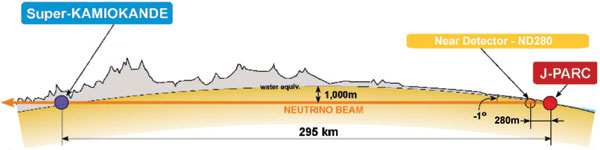
\includegraphics[width=.9\textwidth]{./Figures/t2k-schematic.jpg}
\caption{A schematic of the T2K experiment. The path of the neutrino beam is shown as it travels from the JPARC facility to Super-Kamiokande through ND280 and 295~km of rock. \label{fig:t2k_overview}}
\end{figure}

\subsection{$\nu_\mu$ Beam at JPARC}

The T2K beam is off-axis at $2.5^{\circ}$ with respect to a line drawn from the proton target to the far detector 295~km away. This design choice generates a neutrino beam with a narrow energy band peaking at 600~MeV at the expense of a lower total flux of neutrinos possible in a wide band beam. The choice of energy peak maximizes the probability of $\nu_\mu \rightarrow \nu_e$ oscillation given the baseline of 295~km and maximizes the probability for $\nu_{\mu}$ disappearance. Additionally, Super-K searches for a CCQE-like signal from neutrino interactions and the branching ratio of CCQE interactions is significantly lower at neutrino energies greater than 1~GeV. So the choice of beam peak energy also reduces backgrounds from other neutrino interaction modes. Figure \ref{fig:oabeamflux} shows the $\nu_\mu$ survival probability at 295~km as a function of neutrino energy. It also shows the difference in neutrino flux shape for three off-axis angles. The plots show that the minima of the $\nu_\mu$ survival probability coincides by design with the peak of the neutrino flux at $2.5^{\circ}$ off-axis. In addition, the feedown backgrounds from high energy neutrino interactions are also lowered by having a collimated, low energy neutrino beam.

\begin{figure}
\begin{center}
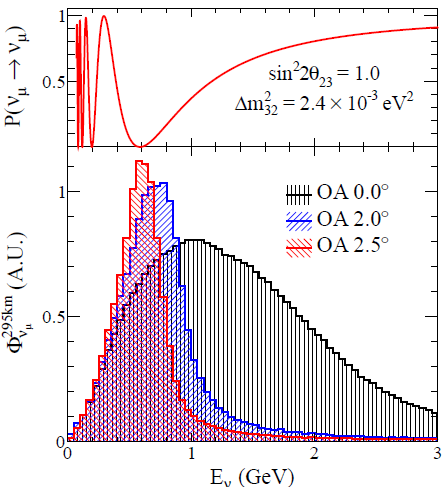
\includegraphics[width=.7\textwidth]{./Figures/OAbeamflux.png}
\end{center}
\caption{The survival probability of a muon neutrino as a function of
  neutrino energy (top) and the shape difference between an on-axis
  and off-axis beam (bottom). Note that the beam energy peaks at 600~MeV at 2.5 degrees off axis. \label{fig:oabeamflux}}
\end{figure}

The JPARC complex has three accelerators that generate the
protons used by the primary and secondary T2K beamlines. First, the
Linear Accelerator (LINAC) accelerates H\textsuperscript{-} to
181~MeV. Second, the Rapid-Cycling Synchotron (RCS) charge strips the
H\textsuperscript{-} to a proton at injection and then accelerates to
3~GeV with a 25~Hz cycle. Finally, the Main Ring (MR) accelerates the
protons to 30~GeV. Five kicker magnets fast-extract these protons from
the MR into 6-8 `bunches' for use in the primary beamline. The bunched
timing structure of the beam allows excellent rejection of non-beam
correlated backgrounds such as cosmic events. The timing is
synchronized between the beam and the rest of the detectors via two
independent GPS modules located at the beam and at Super-K. The timing
is synchronized to an order of 50~ns.

\begin{figure}
\begin{center}
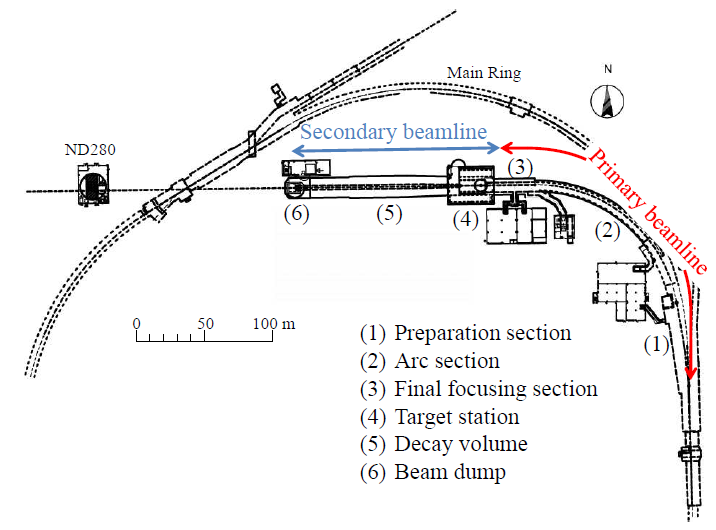
\includegraphics[width=6in]{./Figures/beam1.png}
\end{center}
\caption{A schematic of the primary and secondary beamlines.}
\label{fig:beam1}
\end{figure}

After the MR, the primary beamline points the 30~GeV proton beam towards Super-K while the secondary beamline converts the protons into a focused, 600~MeV $\nu_\mu$ beam. To calculate the expected flux at ND280 and Super-K it is crucial to have precise measurements of the beam timing, direction, profile and proton content. These quantities are measured by four types of monitors placed along the primary beamline.

\begin{enumerate}
\item Beam Intensity Monitor: This monitor consists of 5 current
  transformers (CTs) made of a 50-turn toroidal coil around a
  cylidrical ferromagnetic core. They measure the absolute beam
  intensity with $2\%$ uncertainty and the relative intensity to
  $0.5\%$ fluctuation. 
\item  Beam Position Monitor: Several electrostatic monitors made of
  four segmented cylindrical electrodes surround the proton beam. The
  left-right and top-bottom asymmetry of beam induced current in the
  electrodes is measured to monitor the proton beam center to a
  precision of less than 450~$\mu$m. The tolerance is 500~$\mu$m.
\item Beam Profile Monitor: Protons pass through multiple segmented secondary
  emission monitors (SSEM). Each SSEM is made of horizontally and
  vertically stripped titanium foils 5~$\mu$m thin with a HV anode
  foil between them. Secondary electrons from protons passing through the foils cause current
  in the strips, which is used to reconstruct the beam profile. The
  beam width is measured with 200~$\mu$m uncertainty while the requirement
  is 700~$\mu$m. As there is a $0.005\%$ beam loss from this monitor,
  they are only used during beam tuning.
\item Beam Loss Monitor: Many beam loss monitors consisting of a wire
  proportional counter filled with Ar-CO$_2$ mixture
  measure loss in beam power to a sensitivity of 16~mW.
\end{enumerate}

\begin{figure}
\begin{center}
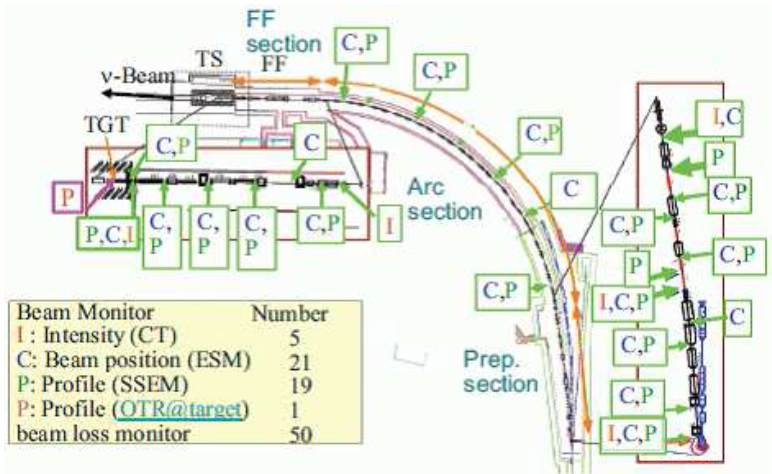
\includegraphics[width=3in]{./Figures/beam2.png}
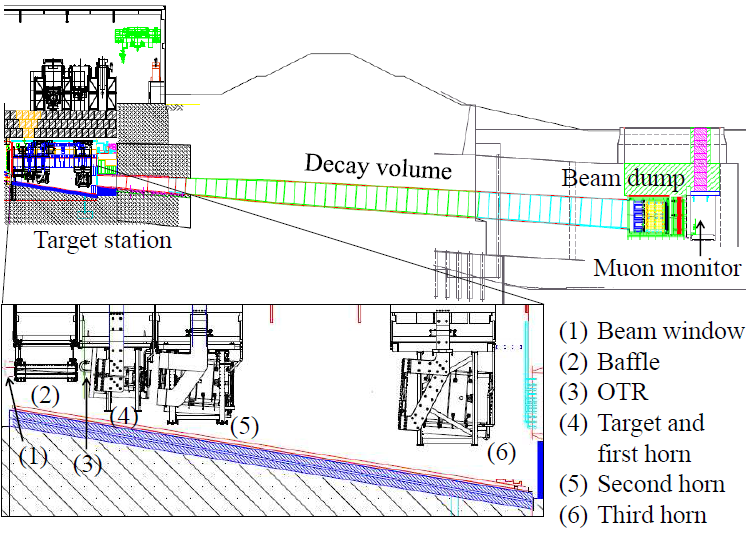
\includegraphics[width=3in]{./Figures/beam3.png}
\end{center}
\caption{A more detailed view of the primary (left) and secondary (right) beamlines. The location of the monitors are shown on the   primary beamline.}
\label{fig:beam2}
\end{figure}
In the secondary beamline, the proton hits a target and generates
pions and kaons. Magnetic horns charge select and focus these
particles that then decay into
neutrinos, yielding the T2K neutrino beam. There are three major
sections: the target station, the decay volume and the beam dump.

The target station has an optical transition radiation (OTR) monitor
to observe the beam profile upstream of the target. The OTR is made of
a thin aluminum foil placed at $45^{\circ}$ to the incident beam. The
foil emits visible light from transitional radiation around where the
beam hits. The light is collected to image the beam profile. Further
downstream in the target station is a 91.4~cm long, 2.6~cm diameter
graphite target with a density of 1.8~g/cm\textsuperscript{3}. This
corresponds to 1.9 interaction lengths. The final elements of the
target hall are three magnetic horns  that generate a 2.1~T toroidal
field for a potential 350~kA of current. The data used in this
dissertation corresponds to a maximum horn current of 250~kA. The
first horn collects while the second and third
horns focus the charged pions and kaons. For optimal
specifications, the increase in the peak of the neutrino flux at Super-K is 16 times
the flux with no magnetic field. The uncertainty of the current in
each horn is $\sim 2\%$ and the uncertainty of magnetic
field strength is $\sim 2\%$ for the first horn and
$\sim 1\%$ for the other two.

Downstream of the target station, a 96~m long steel tunnel provides a
decay volume for charged pions and kaons to decay into neutrinos. The
decay volume terminates at a beam dump positioned 109~m from the
center of the graphite target along the $2.5^{\circ}$ path. It
consists of 75 tons of graphite that stop all hadrons and muons below
5~GeV. Located in the beam dump is the Muon Monitor (MUMON) which
measures the muon profile center to a precision of 3~cm. The
measurement from MUMON provides an added constraint to the neutrino
flux. 

\subsection{Super-Kamiokande Far Detector}

The T2K far detector, Super-Kamiokande, is the world's largest
water-Cherenkov detector located 1~km below Mt. Ikenomiya on the west
coast of Japan. It is a cyclindrical detector filled with 50~kton of
pure water and lined with 13,000 photomultiplier tubes (PMTs). There
were several running periods since Super-K was built with the T2K
experiment taking place during run period SK-IV. 

\begin{figure}
\begin{center}
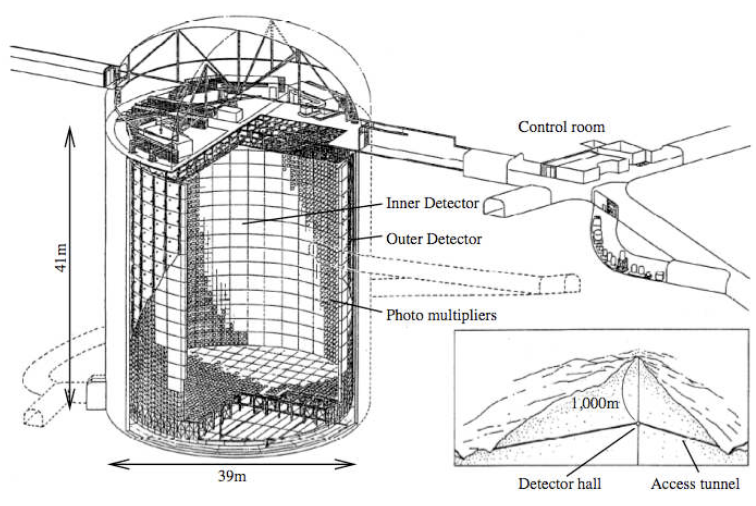
\includegraphics[width=6in]{./Figures/superk.png}
\end{center}
\caption{The Super Kamiokande Detector at the far detector site of
  T2K.}
\label{fig:superk}
\end{figure}

Super-K has two detection volumes, the inner and the outer
detectors. The outer detector (OD) is a cylindrical shell 2~m thick
radially. It is lined with 1885 outward facing
PMTs. The OD primarily serves to veto cosmic background events and
has nearly $100\%$ efficiency. The inner detector (ID) is a cylinder 33.8~m in diameter and 36.2~m in height. It is lined
with 11,129 inward facing, 50~cm diameter PMTs. This yields $40\%$ PMT
cathode coverage with a total $20\%$ light collection efficiency
when combined. Super-K searches for characteristic rings resulting
from Cherenkov light generated by passing charged particles. The ring
properties are used to reconstruct relevant quantities of the
particle. 

\subsection{ND280 Near Detector Complex}

To constrain uncertainties on the neutrino flux as well as neutrino
interaction cross sections, the T2K experiment uses a near detector
complex to observe the beam 280~m downstream of the target. The near detector
site has an iron/scintillator detector (INGRID) placed on-axis with the beam to
monitor the beam profile. A collection of other detectors (ND280) is located
$2.5^{\circ}$ off-axis and is the primary source of neutrino flux and
interaction cross section constraints. 

\begin{figure}
\begin{center}
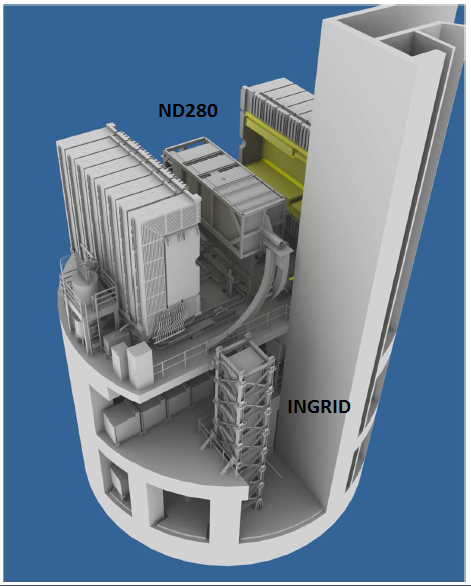
\includegraphics[width=6in]{./Figures/pit.png}
\end{center}
\caption{A model of the near detector complex located in the `pit' at
  JPARC. The off-axis detector ND280 and the on-axis detector INGRID
  are visible.}
\label{fig:pit}
\end{figure}


\begin{figure}
\begin{center}
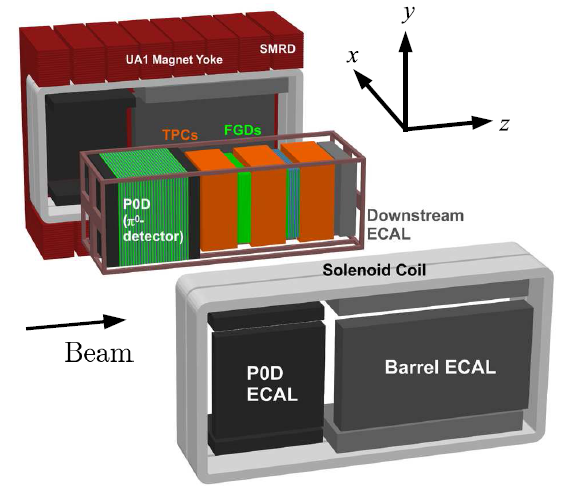
\includegraphics[width=6in]{./Figures/nd280.png}
\end{center}
\caption{A model of ND280 with the major subdetectors color coded.}
\label{fig:nd280}
\end{figure}

The ND280 is a magnetized tracking detector placed inside the recycled
UA1 magnet. It is divided into several sub-detectors, each optimized
for different measurements. Inside the magnet, the most upstream
detector is the Pi-Zero ($\pi^0$) Detector (P0D) consisting of alternating
planes of scintillator bars, sheets of lead/brass radiator, and in the central
region, bags of water. A more detailed decription of the P0D will be provided later. Downstream of the P0D is a tracking detector
comprising of an alternating setup of three Time Projection Chambers
(TPCs) and two Fine Grain Detectors (FGDs). The FGDs are constructed
similar to the P0D but with much smaller scintillator bars for greater
resolution. Surrounding the P0D, TPCs and FGDs and at the most
downstream end of ND280 are three electromagnetic
calorimeters (P0DECAL, barrelECAL and DSECAL respectively) responsible for reconstructing
energy of particles escaping the central detectors. Finally, the
magnet flux return yoke is equipped with planes of scintillator (SMRD)
to constrain external backgrounds and measure sideways muons from neutrino interactions. The entire near detector complex is
located at JPARC in a pit of diameter 17.5~m and of depth 37~m. 

As the analysis in this disseration primarily uses data from the P0D
and the tracking detectors (TPCs and FGDs), they are described in
greater detail. Short descriptions of the other subdetectors are also included.

\subsubsection{$\pi^0$ Detector (P0D)}

The primary goals of the P0D are to measure the rate of neutrino
induced, neutral current $\pi^0$ production on water and the amount of
$\nu_e$ content in the neutrino beam. The P0D is a segmented, scintillation detector with two
major types of regions: the upstream and central electromagnetic
calorimeters (USECAL and CECAL) and the water
target (WT). The water target is nestled in between the USECAL and
CECAL. 

\begin{figure}
\begin{center}
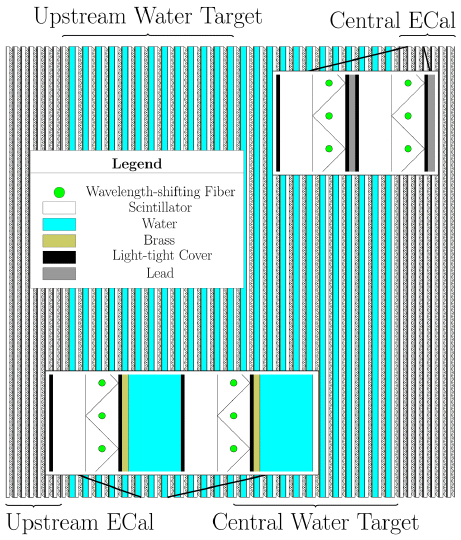
\includegraphics[width=.7\textwidth]{./Figures/p0d1.png}
\end{center}
\caption{A schematic of the entire P0D. The alternating layers of
  lead, brass, scintillator and water are shown as well as the ECAL
  and water target regions.}
\label{fig:p0d}
\end{figure}

The two ECALs are designed to convert photons escaping from the water
target region and provide enough information to reconstruct the energy
of the contained electromagnetic shower. They are made by interleaving
7 ``p0dules'' with 4.5~mm thick sheets of lead radiator. The water
target contains the primary volume for neutrino interactions used in
this analysis. It has 26 ``p0dules" interleaved with 1.28~mm thick
sheets of brass radiator and 28~mm thick water layers. A water layer
consists of two drainable water bags housed in a PVC frame. 

\begin{figure}
\begin{center}
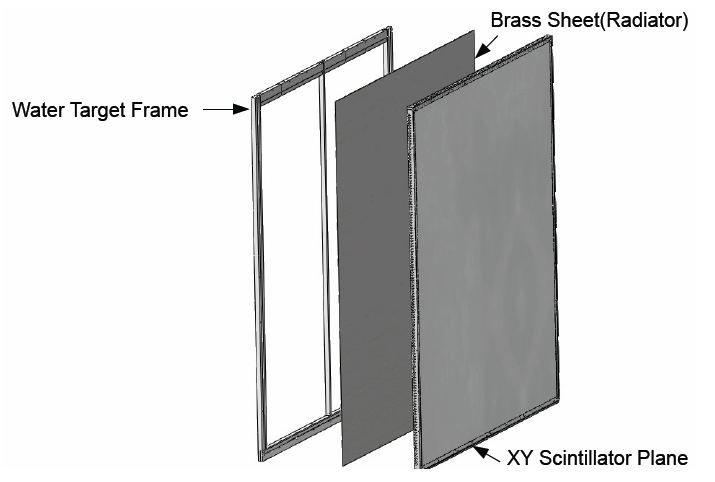
\includegraphics[width=6in]{./Figures/waterp0dule.png}
\end{center}
\caption{An exploded view of a single water target p0dule.}
\label{fig:waterp0dule}
\end{figure}

\begin{figure}
\begin{center}
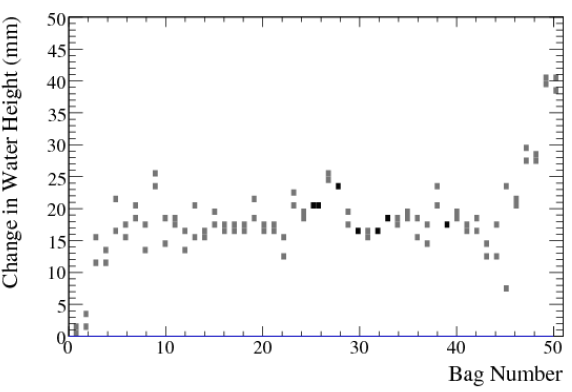
\includegraphics[width=.7\textwidth]{./Figures/waterheight.png}
\end{center}
\caption{The change in height in all water bags over 19 days of
  monitoring. Some settling at the edges is expected and observed, especially near bags 49 and 50 where the P0Dule bulges outward from water pressure.}
\label{fig:waterheight}
\end{figure}

Measuring the water cross section is facilitated by allowing the P0D to collect
data in both water-in and water-out running modes. There are two types of data runs. The water bags are filled
for the water-in running and drained for water-out running. A
statistical subtraction of the two data sets would then yield the neutrino
interaction rates on water only. The mass of the P0D is 15, 800~kg
with water and 12, 900~kg without water. To properly calculate the
neutrino interaction rate, it is crucial to monitor the
amount of water in the P0D at any given time. There are two types of
sensors installed in every water bag: wet/dry binary sensors and pressure depth
sensors. The depth sensors have a measurement uncertainty of $\pm
1$ ~mm. In conjunction with measurements from the external water
storage tank and the surveys of the total P0D dimension, the
uncertainty on the amount of water in the water target region is
constrained to less than $1\%$.

A p0dule is the basic
construction unit for the P0D scitillators and consists of two planes of vertical and horizontal
scintillator glued together. Each scintillator plane is constructed
with a side-by-side array of triangular scintillator bars. The
orientation of the bars for both scintillator planes is perpendicular
to the beam direction. The bars in each plane are also perpendicular
to each other. The scintillator plane with vertically oriented bars is
also referred to as the X-layer and has 126 triangular bars. The
horizontal scintillator plane, the Y-layer, has 134 bars. Each p0dule
is also sandwiched between sheets of high-density polyethlene (HDPE)
and supported by PVC frames.

The scintillator bars are made of polystyrene and co-extruded with a
TiO$_2$ reflective layer. They have a triangular cross section 17~mm
high and 33~mm wide. The outside surface and the two ends are coated
with a TiO$_2$ mix to reflect scintillation light and maximize light
yield in each bar. Each bar has a hole drilled down the center
with a 1~mm diameter wavelength-shifting (WLS) fiber threaded
through. On one end the fiber is coated with a reflective material. On
the other end, the WLS fiber carries scintillation light from the bar
directly to a multi-pixel photon counter (MMPC).

\begin{figure}
\begin{center}
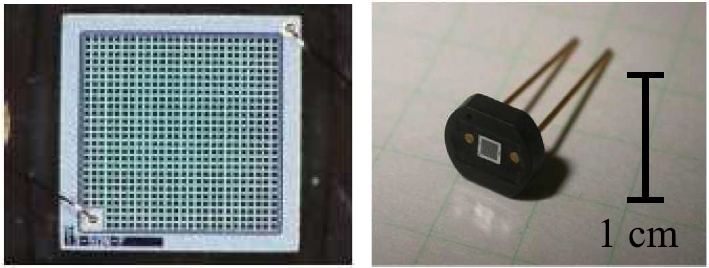
\includegraphics[width=5in]{./Figures/mppc1.png}
\end{center}
\caption{The Hamamatsu MPPCs used in all scintillator detectors at
  the near detector site. The active region of the $1.3\times 1.3$~mm sensor is shown on the left and
  the actual MPPC on the right.}
\label{fig:mppc}
\end{figure}

\begin{figure}
\begin{center}
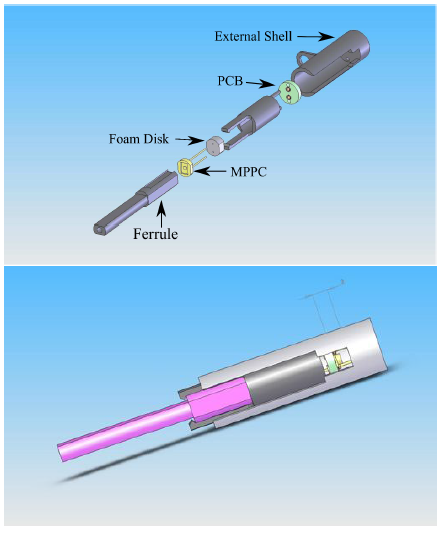
\includegraphics[width=5in]{./Figures/mppc2.png}
\end{center}
\caption{An exploded (top) and assembled (bottom) view of the custom
  optical connectors used to pair an MPPC to the WLS fiber from a
  scintillator bar. These parts were designed and fabricated by CSU.}
\label{fig:mppc}
\end{figure}

There are 10,400 indivdually tested MPPCs installed in the entirety
of the P0D. Due to space constraints for the P0D, the MPPCs are
attached to the WLS fibers immediately at the end of each scintillator
bar using a custom optical connector. These magnetic field immune
MPPCs are manufactured by Hamamatsu and are used for every segmented
scintillator detector in ND280.

\begin{figure}
\begin{center}
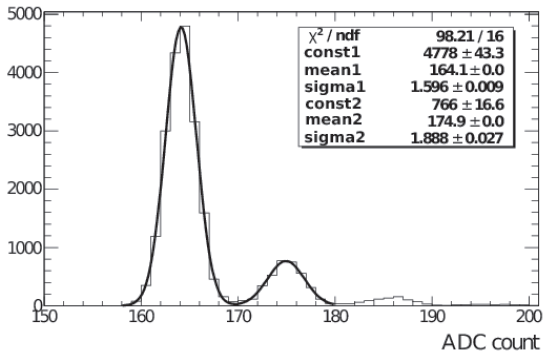
\includegraphics[width=6in]{./Figures/pedestal.png}
\end{center}
\caption{The dark noise ADC spectrum from a single MPPC. The pedestal
  peak and the 1 p.e. peak are shown with gaussian fits.}
\label{fig:pedestal}
\end{figure}

An MPPC has a 1.3~mm by 1.3~mm active detection region of 667 50~micron
pixels. Each pixel runs in Geiger mode and outputs a clean pulse when
an incident photon triggers a cascade. For low light intensities as
expected from neutrino interactions, the probability of multiple
photons landing on the same 50~micron pixel is small. So the number of
pixels fired in each MPPC is a good measure of the total number of
photons incident on the sensor. The dark noise spectrum, i.e. the digitized output from each MPPC
without any input light signal, is used to calculate the pedestal and
the gain for each MPPC. The pedestal is the baseline output from an MPPC when
there is no photoelectron-equivalent (p.e.) signal observed and the gain is
defined as the separation between the pedestal peak and the first
p.e. induced peak. A physics signal is then calibrated by first
subtracting out the pedestal value and then dividing by the gain to
yield the total p.e. corresponding to the collected light. The
expected signal strength is up to a few hundred p.e. for physics
events in the P0D. 

The timing structure of the P0D electronics is designed to reflect the
bunching nature of the neutrino beam. The P0D electronics has 23
cycles per beam spill trigger where each MPPC integrates the observed
charge for a preset period of time. Each intergration cycle is
480~ns long followed by a 100~ns period of electronics dead-time. The
integration cycles are aligned with the 58~ns wide beam bunches so there is no
dead-time with respect to neutrino beam induced interactions. A 2.5~ns
resolution clock time-stamps an MPPC readout that integrates charge
greater than 2.5 p.e. in a single cycle. 


\subsubsection{Tracker (TPCs and FGDs)}

The Tracker, consisting of alternating placements of three time projection chambers (TPCs) and
two fine grained detectors (FGDs), provides high resolution
reconstruction of charged particles. The TPCs in particular can easily
determine the track multiplicity in a physics event, measure the
momentum of a charged track from magnetic field induced curvature and
indentify particle type by the ionization signature. The FGDs
provide target mass for neutrino interactions as well as assist the
TPCs in reconstruction. 

\begin{figure}[h]
\begin{center}
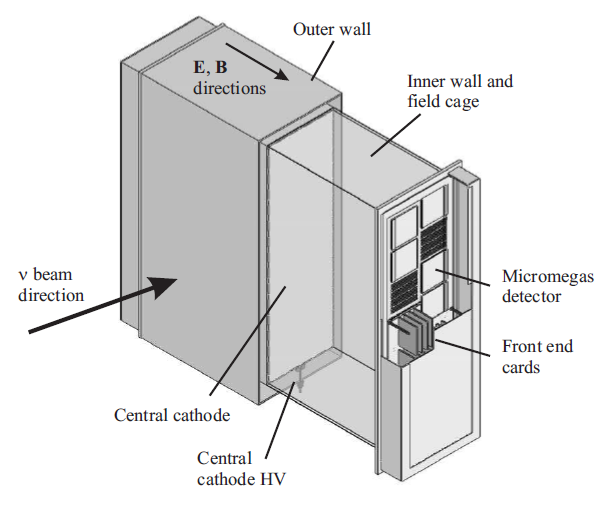
\includegraphics[width=3.6in]{./Figures/tpc1.png}
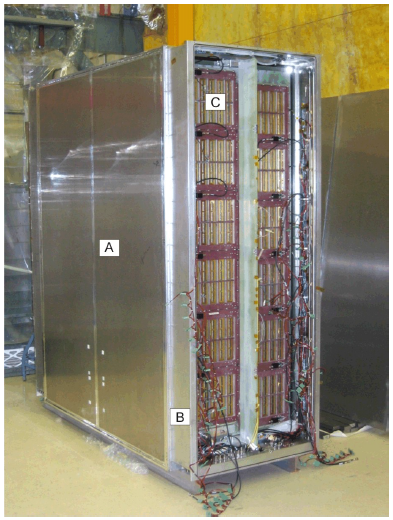
\includegraphics[width=2.4in]{./Figures/tpc2.png}
\end{center}
\caption{A simplified diagram of the TPC (left) and a picture of an
  assembled TPC (right).}
\label{fig:tpc}
\end{figure}

The TPCs consist of an inner and outer box made from copper-clad
aluminum skins. The outer box contains CO$_2$ as an insulating gas and
the inner drift chamber has a 95:3:2 mixture of
Ar:CF$_4$:C$_4$H$_{10}$. A central cathode plane in conjunction with
11.5~mm pitch copper-strip panels generates an uniform
electric field aligned with the ND280 magnetic field. Ionization
electrons drift to one of two readout planes located on either side of
each TPC. 

Each readout plane has twelve 342~mm~$\times$~359~mm Micromegas pads for a
total of 9~m$^2$ coverage over the three TPCs. The micormegas pads
have 7.0~mm~$\times$~9.8~mm segmentation allowing for high resolution
reconstruction of charged tracks and a near $100\%$ detectior
efficiency of minimum ionizing particles such as high energy
muons. The gas mixture in the inner box was chosen for high drift speed and low
diffusion. Each TPC contains 3000~L of the Argon gas mixture and is
maintained under positive pressure.

The two FGDs are similar in structure to the P0D. It is a segmented,
scintillation detector constructed from 9.61~mm~$\times$~9.61mm~$\times$~1864.3~mm
bars of polystyrene. The orientation of the bars follows that of the
P0D with all bars perpendicular to the beam direction. Each bar has a
hole down the middle threaded with a WLS fiber and read-out by
Hamamatsu MPPCs. The FGDs contain 1.1~tons of target material and are
of dimension 2300~mm~$\times$~2400~mm~$\times$~365~mm. The most upstream FGD has 30
scintillator layers of 192 bars per layer. Unlike the P0D, there is no
interleaved radiator material. The downstream FGD mimics the water
target region of the P0D with 7 pairs of scintillator planes
alternating with six 2.5~cm water layers. Though the FGDs can also be
used to calculate water cross sections via statistical subtraction of
event rate, this analysis uses the FGDs and TPCs primarily for their
tracking capabilities. 

\subsubsection{SMRD and Magnet}

A 0.2~T magnetic field is generated for ND280 with a recycled magnet
from the UA1/NOMAD experiments at CERN. Water-cooled aluminum coils
provide a dipole field in the X direction and are mechanically supported by a
850~ton flux return yoke. The yoke is divided into two symmetric
pieces with two aluminum coil segments per piece to allow access to
the inner detectors. A nominal current of 2900~A is provided to the
magnet. The magnetic field inside was mapped using a
computer-controlled movable electronic cards holding three Hall
probes. The mapping procedure was completed at a magnetic field
strength of 0.07~T and later extrapolated to the full 2~T case. The
field strength measurement has an uncertainty of 2~G for each component
which corresponds to a momentum measurement error of $2\%$ for sub-GeV
particles. 

\begin{figure}
\begin{center}
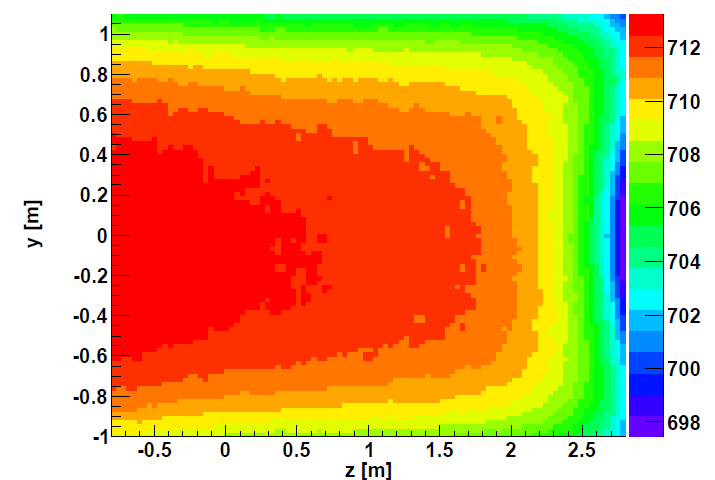
\includegraphics[width=6in]{./Figures/magneticfield.png}
\end{center}
\caption{The mapped magnetic field strength from a 0.07~T survey with
  Hall probes.}
\label{fig:magneticfield}
\end{figure}

\begin{figure}
\begin{center}
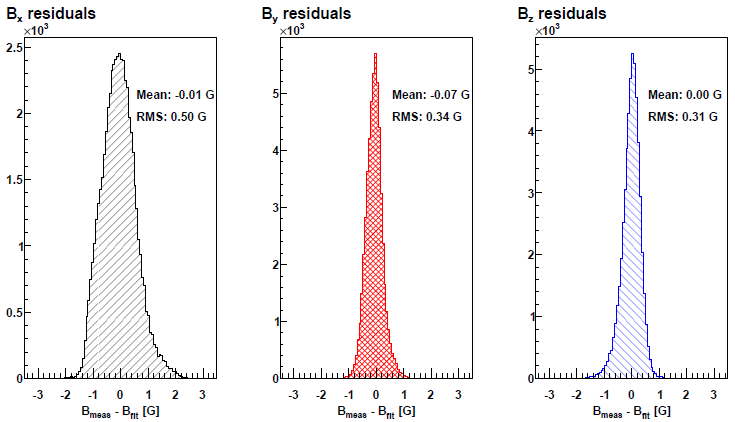
\includegraphics[width=6in]{./Figures/magneticfield2.png}
\end{center}
\caption{The measured value of the magnetic field components in the
  UA1 magnet.}
\label{fig:magneticfield2}
\end{figure}

Several scintillator planes are installed within the flux return yoke
and comprise the Side Muon Range Detector (SMRD). The primary goal of
this detector is to tag escaping particles (mostly muons) from the target volumes of
the inner detectors. It also allows collection of cosmics data by
using coincident activity in different regions of the flux return yoke
to indicate a candidate cosmic track. Finally, it can be used for veto
purposes to reject beam-correlated events occuring on target material outside
the physical ND280 volume. 

\begin{figure}
\begin{center}
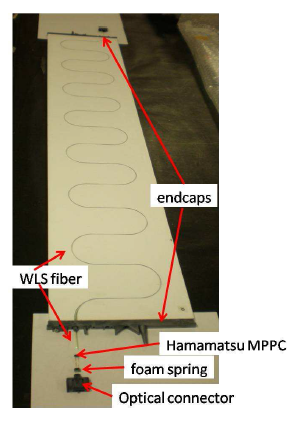
\includegraphics[width=4in]{./Figures/smrd1.png}
\end{center}
\caption{A scintillator plane from the SMRD with the WLS groove shown.}
\label{fig:smrd}
\end{figure}

There are 16 C-shaped pieces to the flux return yoke. Each piece has
fifteen 1.7~cm thin air gaps that contain the SMRD scintillator
volume. The size of each scintillator is matched to the total
available space in the corresponding air gap. Each scintillation plane
has an S-shaped groove cut into one side and lined with WLS fiber. The
fiber is read out on both ends by an MPPC. The plane is also wrapped
in foil to ensure light-tightness. The planes yield around 50~p.e. of
light-yield for a minimum ionizing particle such as a high momentum
muon. Comparing light arrival time for the MPPCs on both ends of a
plane allows a calculation of vertex position to a resolution of
7~cm. 

\subsubsection{Electromagnetic Calorimeters}

There are three electromagnetic calorimeters that surround the inner
detectors. The P0D-ECAL and the barrel-ECAL surround the P0D and the
Tracker respectively while the downstream ECAL (DSECAL) is directly
downstream of the Tracker. The structure of the ECALs mimics the ECAL
regions of the P0D. 

There are 13 independent modules: 6 barrel-ECALs, 6 P0D ECALs and one
DSECAL. Each ECAL consists of planes of scintillator made of
4.0~cm~$\times$~1.0~cm rectangular cross section bars. The bars have an
elliptical hole drilled and threaded with WLS fiber. As with the P0D
and FGD, the ECALs are also read-out with Hamamatsu MPPCs. Some fibers
have readouts at both ends instead of one end having a mirror
coating. Each pair of perpendicular scintillator layers is alternated
with a sheet of lead radiator. 

The DSECAL has 34 scintillator layers with X and Y directional
orientation (perpendicular to the beam direction Z). The barrel-ECAL
31 layers and are oriented parallel to the beam. The bars running
along the Z axis (in the beam direction) are read-out at both ends for
better positional reconstruction. The alternating lead
sheets in the barrel and downstream ECAL are 1.75mm thick. As the P0D-ECAL does
not have the same containment requirements due to the radiator already
present in the P0D, it only has 6 scintillator layers per module
alternated with 4~mm lead sheets. 

\subsubsection{INGRID}

Along with the off-axis sub-detectors, the near detector complex also
houses an on-axis detector called INGRID to monitor the beam direction
and intensity at a 280~m baseline. The total flux on-axis is
significantly higher than at 2.5$^{\circ}$ off-axis, and the observed
number of interactions at INGRID allows a measurement of the beam
center with sub 10~cm precision. 

\begin{figure}
\begin{center}
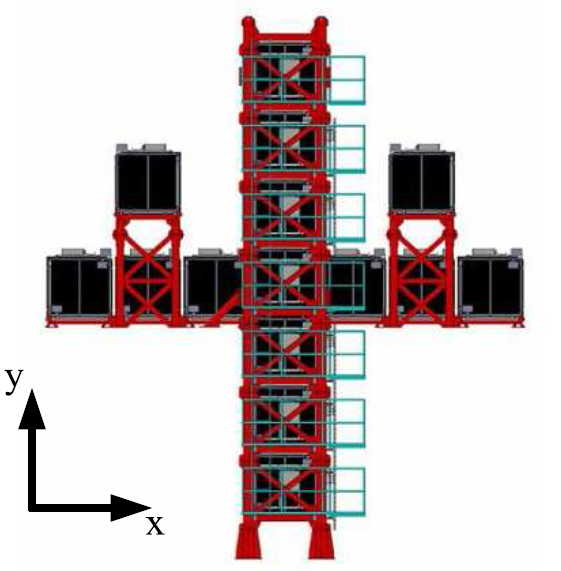
\includegraphics[width=6in]{./Figures/ingrid1.png}
\end{center}
\caption{The INGRID with its 14 cube-like modules assembled as a cross
  and two off-axis modules.}
\label{fig:ingrid1}
\end{figure}

\begin{figure}
\begin{center}
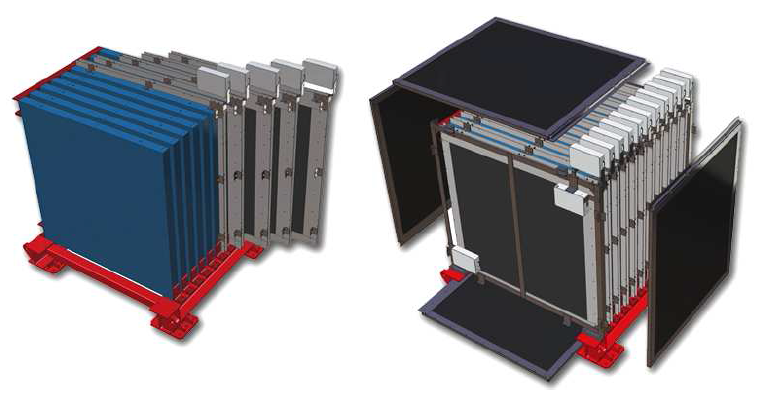
\includegraphics[width=6in]{./Figures/ingrid2.png}
\end{center}
\caption{An exploded view of the structure of a single INGRID module.}
\label{fig:ingrid2}
\end{figure}

INGRID consists of 16 cube-like modules. Fourteen of them are arranged
into a large cross shape with 7 modules per arm and the two central
modules overlapping. The center of the cross is located at the
expected center of the beam. The other two modules are placed slightly
off-axis to measure asymmetry in the beam. Each 7.1~ton module consists of
alternating layers of nine 6.5~cm thick iron plates and 11
scintillator planes. A scintillator plane has 24 horizontal
bars. There are also scintillator planes surrounding and in between each module that
serve as a veto for particles entering from the outside. These veto
planes have 22 scintillator bars each aligned in the beam
direction. INGRID uses the same WLS and MPPC based read-out scheme as
the other scintillator detectors in the near detector complex. An
extra, higher resolution module called the Proton Module was also installed at the beam center
to measure the quasi-elastic channel of charged current neutrino
interactions. 